% For help on subfiles see https://www.sharelatex.com/learn/Multi-file_LaTeX_projects
\documentclass[../main.tex]{subfile}
\begin{document}
	
		\paragraph{} Static analysis is the analysis of a sample without actually executing its code. Various techniques and tools are used like decompiling, string searches, data flow analysis etc. The purpose is to understand the behavior of a malware and sometimes extract some useful intel for dynamic analysis. In this project there are two kinds of static analysis being performed.
		\paragraph{} Frist type of analysis is being performed during or before dynamic analysis to improve code coverage during. It include extracting activites, intent messages(experimental stages), services which are later used as parameters to the android Activity Manager Utitliy to increase code coverage. Have a look to apendix \ref{app::android_am} for more on Activity Manager and how to use it. We will talk about this type in next chapter.
		\todo[inline]{fix reference to appendix}
		
		\paragraph{} Second type of static analysis is performed to extract as much useful information from a sample as possible. The goal of this is to have a lot of information about sample statically analyzed that will be stored in a database and can be used detect similarities between different malware families. We will talk about this type of static analysis in more details in this chapter. For tools, Androguard is used for these analysis because it can be easily automated and had a very rich community support.

		%\todo[inline]{Add info about similarity search to identify malwares or relation between them}
		%\todo[inline]{Add info from http://orbilu.uni.lu/bitstream/10993/26879/1/tr\textunderscore slr\textunderscore article.pdf}
		%\todo[inline]{Add some info about common tools}
		%\subsection{Smali/Backsmali}
		%\paragraph{} smali/backsmali is an assembler/disassembler for the dex format. More detailed information can be found on its github repository \cite{smali/backsmali_github}.
		%\subsection{IDA pro}
		%\subsection{JADX - Dex to Java decompiler}
		% https://github.com/skylot/jadx
		%\subsection{Apktool}\label{sec:apktool}
		%APKTool is one of the major reverse engineering tools for android applications.  \todo[inline]{Add more %info}
		%\subsection{Dex2Jar and jd-gui}
		% dex2jar : https://sourceforge.net/projects/dex2jar/
		% jd-gui : http://jd.benow.ca/
		
		\subsection{Androguard}\label{sec:androguard}
		%\todo[inline]{Introduce androguard}
		%\todo[inline]{MalloDroid, extension of androguard https://www.dfn-cert.de/dokumente/workshop/2013/FolienSmith.pdf}
		%\todo[inline]{Androguard used in http://lilicoding.github.io/SA3Repo/papers/2013\textunderscore guo2013characterizing.pdf}
		\paragraph{} Androguard is an open source tool written in python for analyzing android applications. Its been used in several tools including Virustotal and Cuckoodroid among others. It can process APK files, dex files or odex files. It can disassemble Dex/Odex files to smali code and can decompile Dex/Odex to Java code. Being python based and open source it allows for automating most the analysis process and one can make desired improvements. The analysis is done on need-to basis which means we only use our CPU for the stuff that we need. It has the also the option to be used in interactive mode using androlyze.py script. We will give more information about how to use androgaurd in \ref{subsec:androguard_usage}.
				
		\begin{table} \todo[inline]{Fix the position of table}
			\begin{center}
				\begin{tabular}{|p{5cm}|p{5cm}|}
					\hline \textbf{Classes for Parsing} & \textbf{Classes for Analysis}\\ \hline
					\begin{itemize}
						\item \textbf{APK} Used for accessing all elements inside an APK, including information from Manifest.xml like permissions, activities etc.
						\item \textbf{DalvikVMFormat}	It parses the dex file and gives access classes, methods, strings etc. defined inside the dex file.
						\item \textbf{ClassDefItem} Class for interacting with class information inside the dex file.
						\item \textbf{EncodedMethod} Class for interacting with method information inside the dex file. 
						\item \textbf{Instuction} Class for interacting with instructions, it contains mnem, opcodes etc. Its a base class and a androguard derive a class for each instruction format from this class.
					\end{itemize}
					
					&
					
					\begin{itemize}
						\item \textbf{Analysis} Its the main analysis class and contain instances of all other analysis classes discussed below. create\textunderscore xref() method needs to be called after an instance of this class is created to populate all defined fields in this class.
						\item \textbf{ClassAnalysis} This class contain analysis data of a class like cross references and external methods etc.
						\item \textbf{MethodAnalysis} Contain analysis information of a method like the basic blocks it is composed of etc.
						\item \textbf{DvmBasicBlock} Represents a simple basic block of a method. It contains information about that basic block like its parents, children etc.
						\end{itemize}\\ \hline
					
				\end{tabular}
			\end{center}
			\caption{Some classes of androguard and their description}
			\label{table:androguard_classes}
		\end{table}
		
		\subsubsection{Androguard usage example}\label{subsec:androguard_usage}
			\paragraph{} As we mentioned above, androgaurd can be used in two way, its a good idea to start with interactive CLI mode of androguard just to get some idea of what it is capable of. You can use the below command in your terminal to start the interactive shell. It will import all the required androguard packages and you can start analyzing APKs right away. Depending on how you installed androguard, you may need to execute androlyze.py or just androlyze.
				\begin{lstlisting}[language=bash, xrightmargin = 0.7\textwidth]
					androlyze -s
				\end{lstlisting}
			\paragraph{} This will open a python interactive shell and you can now specify the APK file as show below:
				\begin{lstlisting}[language=python]
					apk, dvm, dx = AnalyzeAPK("path/to/app.apk")
				\end{lstlisting}
			\paragraph{} The analyzeAPK method returned three objects. These classes are also mentioned in \ref{table:androguard_classes}. The first returned class is an object of APK class. This one can be used to get information about the APK most of which are extracted from manifest.xml file. Below is the example on how to extract some information:
			
				\begin{lstlisting}[language=python]
					user@workstation:~$ androlyze.py -s
					Androguard version 3.1.0
					In [1]: pwd
					Out[1]: '/home/user'
					
					In [2]: apk, dvm, dx = AnalyzeAPK("/home/user/workspace/apps/evasion.apk")
					
					In [3]: apk.get_activities()
					Out[3]: [b'com.ouz.evasion.EvasionMainActivity']
					
					In [4]: apk.get_permissions()
					Out[4]: []
					
					In [5]: apk.get_libraries()
					Out[5]: []
					
					In [6]: apk.get_package()
					Out[6]: 'com.ouz.evasion'
					
					In [7]: apk.get_max_sdk_version()
					
					In [8]: apk.get_min_sdk_version()
					Out[8]: '14'
					
					In [9]: apk.get_files()
					Out[9]: 
					['res/layout/activity_evasion_main.xml',
					'res/menu/evasion_main.xml',
					'AndroidManifest.xml',
					'resources.arsc',
					'res/drawable-hdpi/ic_launcher.png',
					'res/drawable-mdpi/ic_launcher.png',
					'res/drawable-xhdpi/ic_launcher.png',
					'res/drawable-xxhdpi/ic_launcher.png',
					'classes.dex',
					'META-INF/MANIFEST.MF',
					'META-INF/CERT.SF',
					'META-INF/CERT.RSA']
				\end{lstlisting}
			\paragraph{} There are a lot of methods that can be called on the APK object, to see them just type "apk." in the CLI and then press tab. The auto-complete feature will show you all the possible methods you can call. For more details you can have a look at the source code or the documentation for this class.
			
			\paragraph{} The dvm class represent DalvikVMFormat class, which basically parse the dex file contained inside the apk and gives us information about the classes, methods, Basic Blocks and instructions.
				\begin{lstlisting}[language=python]
					In [12]: type(dvm)
					Out[12]: androguard.core.bytecodes.dvm.DalvikVMFormat
				\end{lstlisting}
			\paragraph{} In below script we will demonstrate how to get name of some of the methods using this dvm object:
				\begin{lstlisting}[language=python]
					In [13]: methods = dvm.get_methods()[10:15]
					
					In [14]: for method in methods:
					...:     print(method.get_name())
					...:     
					getSettingsActivityName
					<clinit>
					<init>
					capabilityToString
					feedbackTypeToString
				\end{lstlisting}
				
			\paragraph{} The auto-complete feature, documentation or source code can be used in similar way as mentioned above to discover more features more methods or fields of this objects. The dx object is an instance of Analysis class which also provide access to analysis parts classes and methods like cross references, string analysis as shown below:
				\begin{lstlisting}[language=python]
					In [23]: for key in dx.get_strings_analysis():
					...:     print(key)
					...:     
					Unable to create files subdir 
					
					mCommitted=
					mDeliveredData=
					Resolving type 
					No fake drag in progress. Call beginFakeDrag first.
					android.app.Notification$Action
					mAvailIndices: 
					; boundsInScreen: 
					RemoteInput
					Can't change tag of fragment 
					mAvailBackStackIndices: 
					Couldn't fetch mRecreateDisplayList field; dimming will be slow.
					Operations:
					is not a sliding drawer
					NULL
					mRetaining=
					command cannot be null or empty
					mAccessibilityDelegate
					mProcessingChange=
					op #
					Callback may not be null
					onCreateView: id=0x
					.
					.
					.
					.
					 => 
					 : 
					 Unable to instantiate fragment 
					 onLoadComplete: 
					 android:fragment:
					 icon
					 .
					 , tag 
					 Can not perform this action after onSaveInstanceState
					 mediaSession is not a valid MediaSession object
					 mMenuVisible=
					 tag must not be null or empty
					 
				\end{lstlisting}
			\paragraph{} Below script demonstrates how to further examine the results provided by Analysis class object dx.
				\begin{lstlisting}[language=python]
					In [30]: string_analysis = list(dx.get_strings_analysis().values())[10]
					
					In [31]: string_analysis.get_orig_value
					Out[31]: <bound method StringAnalysis.get_orig_value of <androguard.core.analysis.analysis.StringAnalysis object at 0x7fd6247ff7b8>>
					
					In [32]: string_analysis.get_orig_value()
					Out[32]: "Can't change tag of fragment "
					
					In [33]: string_analysis.get_xref_from()
					Out[33]: 
					{(<androguard.core.analysis.analysis.ClassAnalysis at 0x7fd62588d320>,
					<androguard.core.bytecodes.dvm.EncodedMethod at 0x7fd626197b00>)}
					
					In [35]: string_analysis.get_value()
					Out[35]: "Can't change tag of fragment "
					
				\end{lstlisting}
				
			\paragraph{} We encourage reader to play with the androguard interactive CLI. After you have some idea of what can you do, then you proceed to write some python scripts and automate some of the tasks. In section \ref{sec:androgaurd_static_analysis} we will talk about the information that we extracted from APK files using androgaurd.
			
		
		\subsection{Information Extracted from an APK using Androguard}\label{sec:androgaurd_static_analysis}
		\paragraph{} Before getting into details, we would like to mention that the information we extract will be stored in a database and similarity search would be performed on this data to figure out its relations other malware or goodware samples. The more information we have about an APK, more relations we can figure out.
		\paragraph{} Now coming towards, the extracted information, we divide it into different groups as shown in figure \ref{fig:info_extracted}.
		
		\begin{figure}
			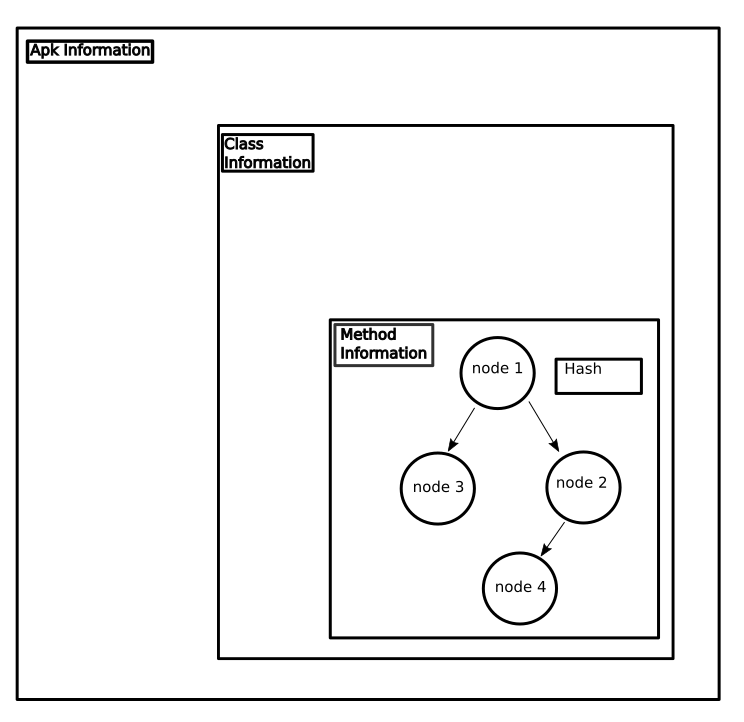
\includegraphics[width=\textwidth]{information_extracted.png}
			\caption{Groups of information extracted using APK}
			\label{fig:info_extracted}
		\end{figure}
		
		
		\begin{itemize}
			\item \textbf{APK information} This contain general information about the APK like Permissions, Package name, Libraries, Certificates, components (activities,services, receivers) and information about all classes contained in this APK. We also wrote some code to extract strings from layout files and other binary xml files contained in the APK. Most of Malwares bitcoin wallet addresses were hard coded in the those files. Figure \ref{fig:apk_info} shows this part of information extracted from an apk and stored in JSON format.
			\begin{figure}
						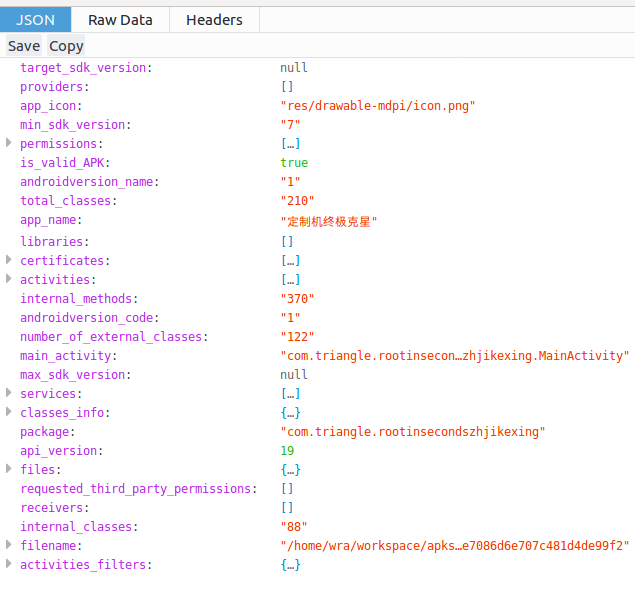
\includegraphics[width=\textwidth]{apk_info.png}
						\caption{APK info}
						\label{fig:apk_info}	
			\end{figure}
			
			\item \textbf{Class information} It represent a single element of the class\textunderscore dictionary contained in APK information. It contains information like fields in the class, its access flags, name, superclass name, number of internal methods, inherited methods etc. It also contain information about methods which are part of this class in the form of a list. Figure \ref{fig:class_info} shows this part of information extracted from an apk and stored in JSON format.
			\begin{figure}
				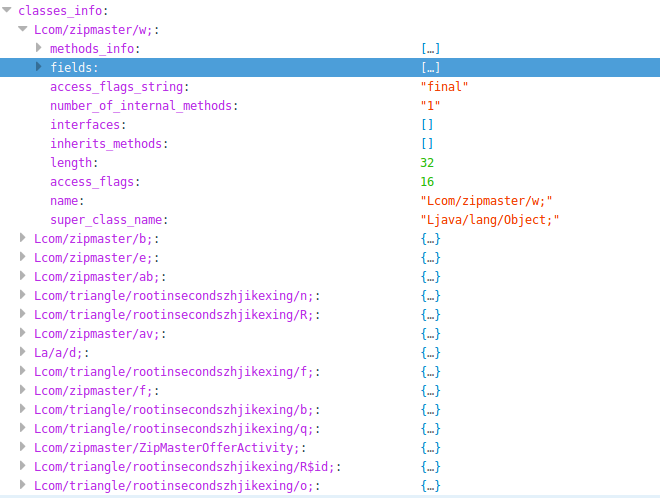
\includegraphics[width=\textwidth]{class_info.png}
				\caption{Class info}
				\label{fig:class_info}	
			\end{figure}
			
			
			\item \textbf{Method information} A we said above, class\textunderscore information contain a list of methods\textunderscore info. Each element of that list contain information about a method such as method name, class name, address, method descriptor, length of method, its cross references, shorty descriptor, Java decompiled source code for that method, Control flow graph of that method and the calculated hash for this method. Figure \ref{fig:method_info} shows this part of information extracted from an apk and stored in JSON format.
			\begin{figure}
				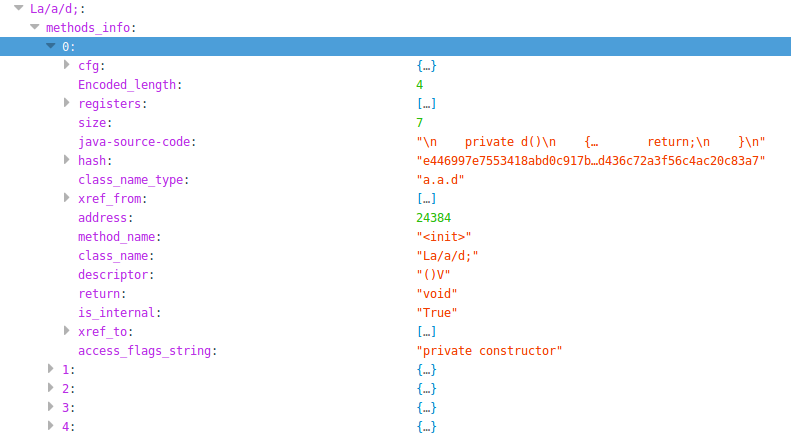
\includegraphics[width=\textwidth]{method_info.png}
				\caption{Method info}
				\label{fig:method_info}	
			\end{figure}
			\item \textbf{Control Flow Graph} Control flow graph contain edges and nodes. Nodes are basic blocks and are basically a list of instructions. Figures \ref{fig:nodes_info} and \ref{fig:edges_info} shows this part of information extracted from an apk and stored in JSON format.

			\begin{figure}
				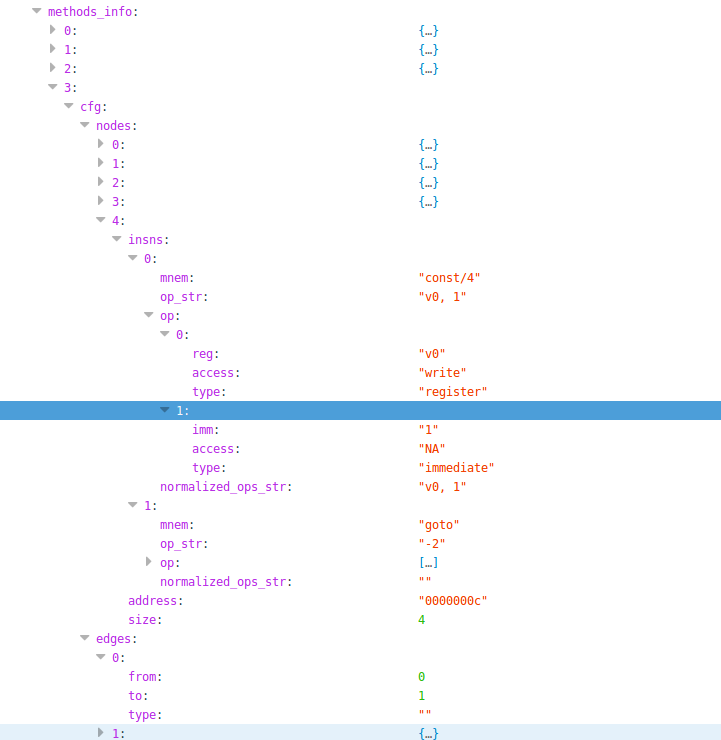
\includegraphics[width=\textwidth]{nodes.png}
				\caption{Nodes info}
				\label{fig:nodes_info}	
			\end{figure}

			\begin{figure}
				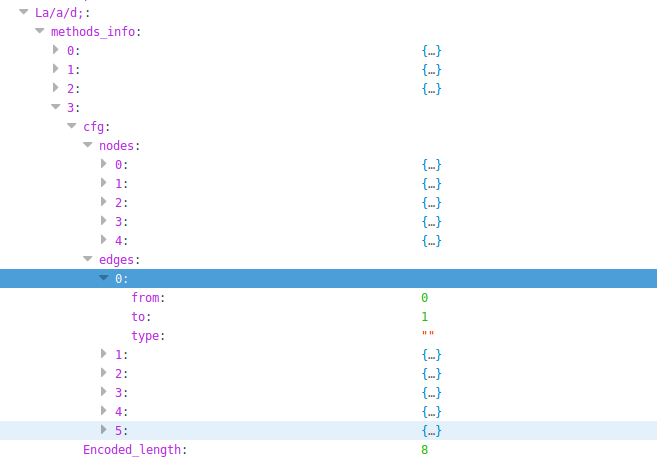
\includegraphics[width=\textwidth]{edges.png}
				\caption{Edges info}
				\label{fig:edges_info}	
			\end{figure}
		

			\item \textbf{Canonical Certificate} In order to compare two control flow graphs, we need to find the Canonical form of this Control flow graph. Fore more details about the topic readers are encouraged to search the Internet for "Graph canonization" and also have a look at the webpage of "bliss" \cite{bliss}. We used pybliss python library \cite{bliss} \cite{junttila2007engineering} to get the canonical certificate of this graph. Before computing this certificate, the smali instructions are normalized according to a specific criteria so that compilation specific changes are ignored like offsets etc. It can be seen in Figure \ref{fig:hash_info}.
			\begin{figure}
				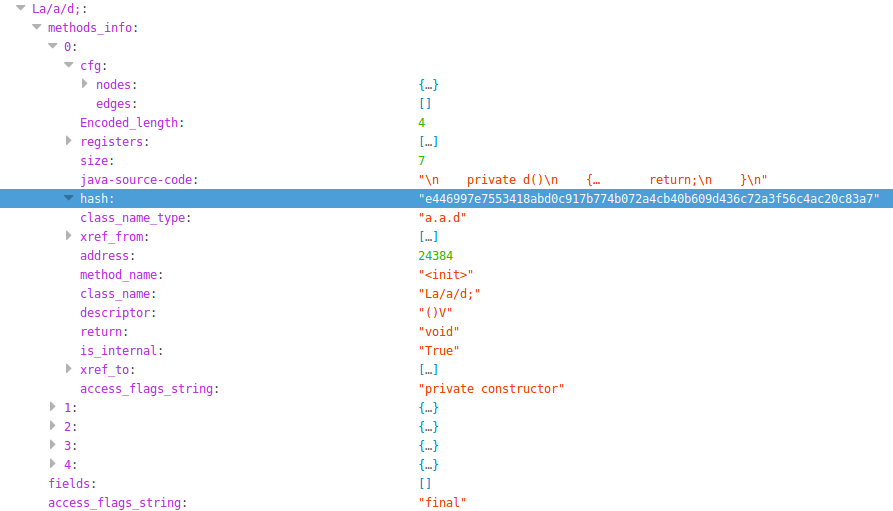
\includegraphics[width=\textwidth]{hash.png}
				\caption{Canonical Certificate}
				\label{fig:hash_info}	
			\end{figure}
		\end{itemize}
		
		\subsubsection{Example usage}
		\paragraph{}Just to make the usage of this extracted data more clear. In this example we process some of the sonicspy samples and tried to figure out how much code they share. We analyzed 16 samples and the result is shown in figure \ref{fig:sonicspy_freq}.
		
		\begin{figure}
			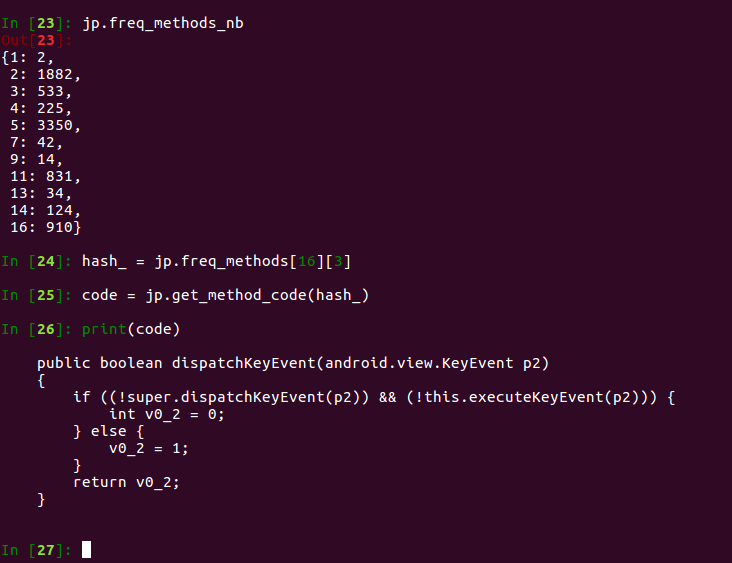
\includegraphics[width=\textwidth]{sonicspy_freq.png}
			\caption{Reused methods in sonicspy variants}
			\label{fig:sonicspy_freq}
		\end{figure}
		\paragraph{} Line 23 in figure prints the result, in this dictionary keys represent frequency or number of samples in which a method is used. Value represent numbers i.e, number of all such methods that has been used in "key" samples, or number of all methods with corresponding frequency. From this analysis we can see that a large portion of code is common between these samples but also that all of this code is not malicious. Most of it is standard android API methods and non-malicious general purpose methods like wrappers etc. It would be very interesting to identify and separate API code from this chunk. It can be topic for further research to identify common non-malicious pieces of code to make analysis easier. \todo[inline]{Add to future work}

		\paragraph{} In the code snippet, "jp" is an object of a class JasonParser which we wrote just to verify information extracted from APKs. In line 24 we get the hash of a specific method and in line 25 and 26, we print its Java source code. Here we can see that its a very general method and its been used in all of the 16 samples analyzed.
		
		\paragraph{} Figure \ref{fig:sonicspy_graph} shows the code reuse graphically. Here we still have the same problem that we can't separate standard API code and malicious parts of code. Figure \ref{fig:sonicspy_graph} was result of processing following samples:
		\begin{itemize}
			\item 9a6b7418729d0b6dc22e8e4925006c6567b303a9
			\item 5a341606fc391d669f1c01c5dd7e93fc49dca0d7
			\item ed84300fb1ba7feef63351e49ddd2930f865bea9
			\item 515453379a26d19c49e60edb8affd801b6001234
			\item ea9079c800cf8d77cccdc393de1d7366b00ba7ec
			\item 96548a4054aa1c798a8318302ab416cdbbedd5bb
			\item 82bc64931d5e86d02792685141da0cfc5fcf147a
			\item 275b55b2addb08912d973a6e181fd70e6bbe5d90
			\item a8b3013c4998196672967028f5612f73c0be23ef
			\item 7bd0f90e75941939671e430f960674c566f7167c
			\item 9f69841f38501e4e527d4563d97838c21006083c
			\item 3f33367040dc423ff97aab7196aa6748ff11cc45
			\item b22f7611916ff2c57514bc40e59924268fb64452
			\item 9d2aa0bcecaf564eb06238086c53ce56e8ca1bf4
			\item 29967d4afd2e11beb85e2f7eec5ce4c1778026a2
		\end{itemize}
		
		\begin{figure}
			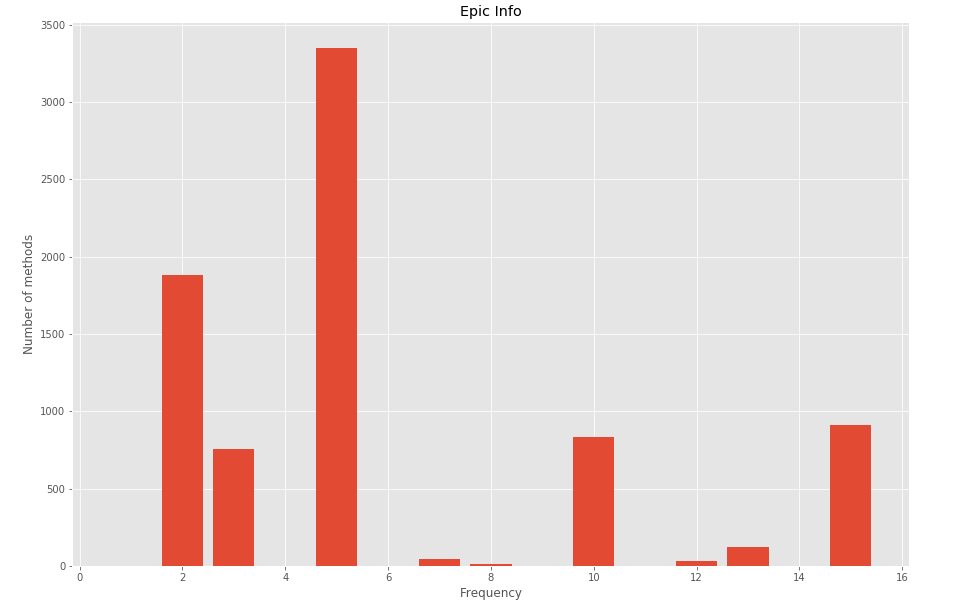
\includegraphics[width=\textwidth]{sonicspy_code_reuse.png}
			\caption{Reused of methods in sonicspy variants}
			\label{fig:sonicspy_graph}			
		\end{figure}
		
		
		\subsection{Chapter Conclusion} In this chapter we discussed the information extraction that can be used to find similarities between different samples. During the course of this work we also identified some bugs in androguard and communicated them to the maintiners of the official github androguard repository \cite{desnos2017androguard}. Example of these are issues number 324, 325, 529, 329. I really appreciate the maintainers of github for their quick responses especially reox \cite{reox}.
\end{document}